\chapter{Ethereum: Sviluppo di applicazioni decentralizzate}
\label{ch:ethereum}

Seguendo la divisione in tre strati di concetti, implementazioni e istanze, definita fin dall'inizio del lavoro, in questo capitolo verrà affrontato l'aspetto implementativo, nel caso concreto della piattaforma Ethereum. I concetti spiegati fino a questo punto possono costituire una base decisionale, un punto di partenza per scegliere le implementazioni che meglio si adattano alle proprie necessità. Possono essere visti come una sorta di contenitore aperto da cui è possibile “pescare” le componenti concettuali da implementare con i relativi pro e contro a seconda degli obiettivi delle applicazioni finali. 

Importante sottolineare che lo stato dell'arte delle blockchain limita l’utilità di descrivere in dettaglio un certo numero di implementazioni concrete. Questa affermazione deriva dal contesto attuale, le blockchain nonostante non siano più definibili come una tecnologia fra le più recenti in confronto alle tempistiche del settore informatico, generalmente non hanno raggiunto una stabilità sufficiente. Usando la terminologia presente nelle analisi e predizioni annuali condotte dalla Gartner\footnote{Gartner è una società di consulenza nel campo dell'Information Technology. Effettua analisi e ricerche al fine di produrre previsioni attendibili per i vari processi decisionali e di investimento.} la blockchain si trova attualmente sulla via di uscita dal cosiddetto "\emph{hype cycle}"\footfullcite{gart2016} \smallskip \footfullcite{gart2018}. Una metodologia usata per rappresentare la maturità, l'adozione e l'applicazione di nuove tecnologie.

\begin{figure}[H]
\centering
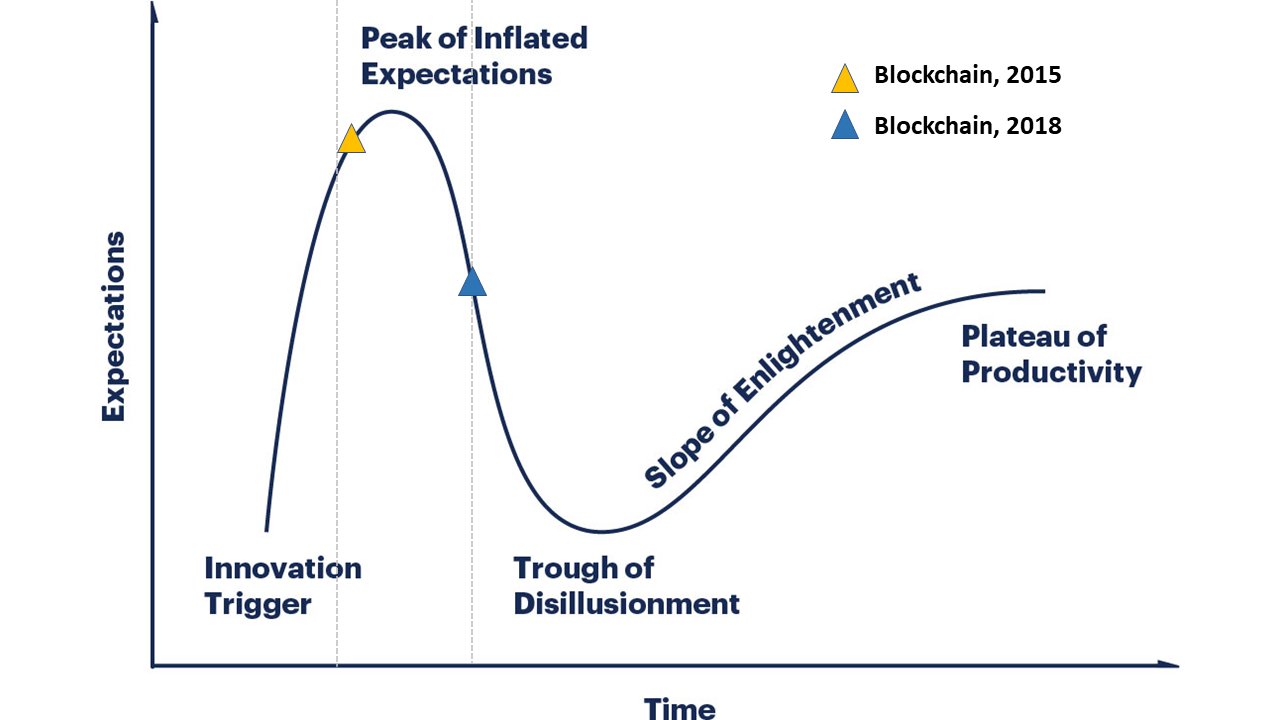
\includegraphics[width=1\textwidth]{immagini/blockchainHype.png}
\caption{Tecnologia blockchain: Hype Cycle}
\label{fig:HypeCycleBlockchain}
\end{figure}

La situazione in figura \ref{fig:HypeCycleBlockchain}, può essere vista come un contesto variabile, di continuo sviluppo con l’emergere di nuove implementazioni, piattaforme e applicazioni. Si tratta di una ricerca spesso finalizzata al miglioramento e all'adozione delle nuove tecniche per contrastare le limitazioni attuali del paradigma blockchain, in una situazione, qual è quella presente, in continuo mutamento e caratterizzata dall'instabilità e in alcuni casi da cambiamenti radicali. Tuttavia, questo non pregiudica l’utilità delle cose dette finora in quanto si tratta di concetti fondamentali che, nel caso peggiore, possono servire anche per comprendere le scelte e gli sviluppi futuri della tecnologia.

La scelta di Ethereum come sistema da presentare, collegato alla successiva costruzione di un’applicazione nel capitolo successivo è stata fatta seguendo tra le altre, queste motivazioni di stabilità, di sviluppo e di innovazione. Viene perseguita l'idea legata alla correlazione tra il successo e la popolarità di un sistema, misurata tenendo conto del numero di partecipanti e di sviluppatori coinvolti, degli strumenti di sviluppo messi a disposizione e dal loro grado di maturità. Si è tenuto conto, anche della frequenza di aggiornamenti e dell’interesse della comunità, degli enti pubblici e privati con i relativi rischi connessi. Un insieme di fattori che le nuove implementazioni dovranno cercare di raggiungere per attrarre nuovi utenti e sviluppatori ai loro sistemi. Al momento dello scrivere la piattaforma Ethereum è il sistema più sviluppato sotto questi aspetti anche grazie all'integrazione di strumenti per la costruzione di applicazioni decentralizzate.

\section{Implementazione Ethereum}

Ethereum è una piattaforma di sviluppo delle applicazioni decentralizzate basata sulla tecnologia blockchain, pubblica e open-source.

La novità principale è data dalla presenza di un linguaggio di programmazione Turing completo. Si tratta dunque, di una blockchain programmabile con un linguaggio chiamato Solidity, attraverso cui è possibile esprimere qualsiasi algoritmo esprimibile con altri linguaggi di programmazione universali. Questi programmi scritti e compilati all’interno della blockchain prendono il nome di “\emph{Smart Contracts}” e si comportano come dei contratti veri e propri. In rapporto ai loro corrispettivi tradizionali i termini contrattuali non sono definiti usando un linguaggio legale, ma direttamente il codice dei programmi (chiamati appunto contratti). Gli smart contracts permettono l’implementazione della logica delle transazioni e la disintermediazione tra le parti interessate grazie ai concetti che guidano le blockchain. 

Riassumendo, la visione del progetto Ethereum è quella di creare un computer decentralizzato permanente e autosufficiente, in grado di resistere ai tentativi di censura. Dal punto di vista della programmazione, nella figura \ref{fig:ArchitetturaBlockchain} è rappresentato il flusso relativo all’architettura delle applicazioni blockchain.

\begin{figure}[H]
\centering
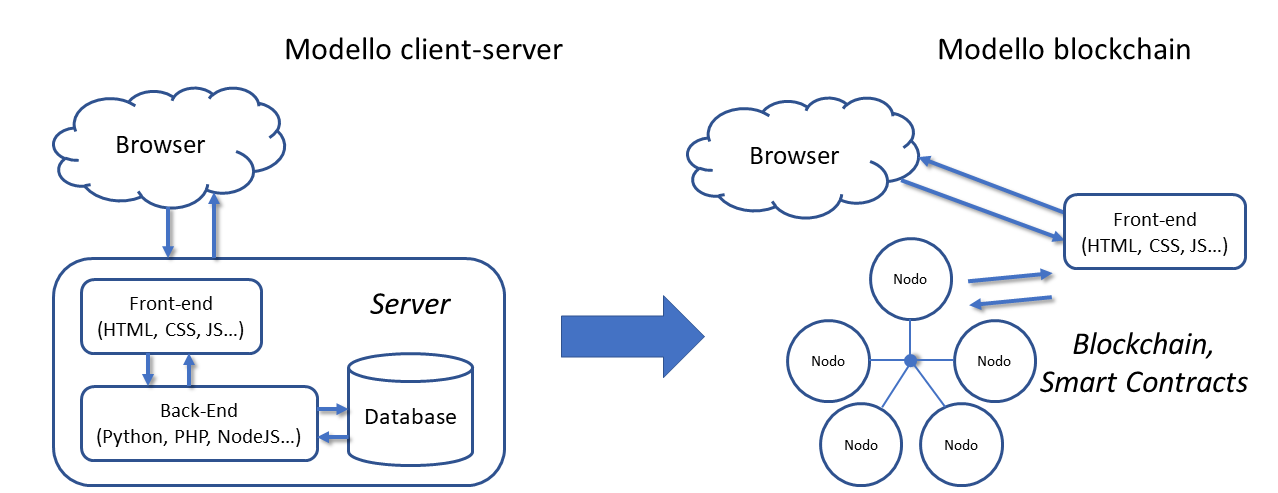
\includegraphics[width=1\textwidth]{immagini/architetturav1.png}
\caption{Architettura blockchain}
\label{fig:ArchitetturaBlockchain}
\end{figure}

In relazione al classico modello client-server nel modello decentralizzato lo strato back-end è direttamente implementato nella blockchain attraverso gli smart contracts. L’esecuzione della logica dei contratti avviene grazie alla macchina virtuale Ethereum (EVM) eseguita da ciascun nodo della rete estendendo così il concetto di database distribuito con la nozione di calcolo distribuito (distributed computing\footfullcite{wikidistrComp}). Ethereum prevede un meccanismo di incentivi incorporato nel sistema di consenso della rete attraverso l’uso di una criptovaluta chiamata Ether. La logica transazionale (estesa con i smart contracts) in relazione alla complessità di calcoli computazionali è regolata da un costo espresso in unità di Gas corrispondente a una frazione di Ether. Si tratta di un meccanismo grazie al quale è possibile prevenire lo spam dovuto ad esempio all’esecuzione di programmi non terminabili.

In questo capitolo verranno analizzate queste modifiche ed espansioni della blockchain Ethereum.

\subsection{Transazioni}

Le transazioni in Ethereum sono estese con tre nuove proprietà:

\begin{itemize}
\item Un campo di dati opzionale
\item Un valore Start Gas
\item Un valore Gas Price
\end{itemize}

In riferimento alle transazioni del capitolo precedente (come ad esempio quella in figura \ref{fig:TransazioneToken}) queste proprietà vengono aggiunte ai campi già descritti precedentemente: mittente, destinatario e valore da trasferire. Le nuove proprietà o campi sono strettamente legati al funzionamento della EVM che può accedere ai campi della transazione.

In particolare il campo di dati (opzionale) può essere usato per identificare specifiche operazioni sulla blockchain come ad esempio la registrazione di domini. Prima di andare avanti è opportuno spiegare che Ethereum prevede due tipi di account, quelli appartenenti agli utenti e ai contratti. Questi account posseggono le stesse caratteristiche. Sono identificati da un indirizzo, mantengono il bilancio di token disponibili e così via, funzionano alla stessa maniera con l’eccezione che i primi (account utente) sono controllati da chiavi private (quindi utenti veri e propri) e gli altri dal codice eseguito in maniera automatica. Proprio per la necessità di eseguire programmi equivalenti al codice dei contratti, sono state create le proprietà Start Gas e Gas Price. Start Gas rappresenta il numero massimo di passi (\emph{step}) computazionali che la transazione a cui si riferisce può eseguire. Gas Price, rappresenta il costo che il mittente è disposto a pagare per l’esecuzione dei programmi. Di solito l’incremento di quest’ultima proprietà permette di conquistare una certa priorità nel processo di validazione delle transazioni\footfullcite{ethWhitepaperTx}.

Come già introdotto, i valori Start Gas e Gas Price permettono di rimediare ai problemi relativi all'esecuzione di programmi infiniti e la conseguente congestione della rete dovuta a un numero eccessivo di calcoli computazionali costosi.

\subsection{Patricia Trees}
% --- da migliorare
La struttura dati usata in Ethereum prende il nome di Patricia Tree (o trie) e rappresenta un’estensione di Merkle Tree (per la definizione si rimanda al capitolo 2.3). Se per lo strato concettuale i Merkle Tree servivano fondamentalmente per la memorizzazione e la verifica delle transazioni attraverso procedimenti di hashing ricorsivi, in Ethereum sono usati anche per memorizzare lo stato della rete e il risultato delle transazioni. In particolare in un blocco della rete al posto di una radice di Merkle Tree (tx root), sono incluse le seguenti tre radici di Patricia Tree:

\begin{itemize}
\item Radice dello stato
\item Radice delle transazioni
\item Radice delle ricevute (delle transazioni)
\end{itemize}

Analogamente a quanto detto per i Merkle Trees, in Patricia Trees grazie all'applicazione ricorsiva di funzioni hash crittografiche (in Ethereum viene usato lo standard SHA-3\footfullcite{sha3Wiki} e in particolare l'algoritmo Keccak256) la radice diventa una sorta di impronta digitale per l'intera struttura dati sottostante. Ogni modifica a qualsiasi livello della struttura farà cambiare il risultato dell'applicazione di funzioni hash sul ramo interessato dalla modifica fino alla radice stessa. 

\begin{figure}[H]
\centering
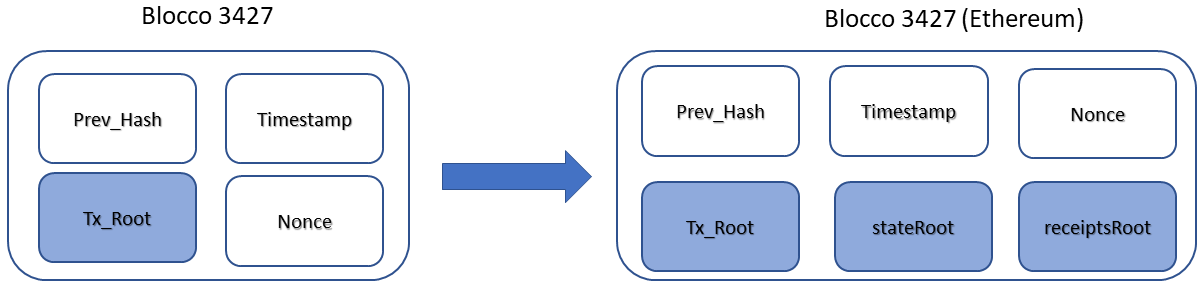
\includegraphics[width=1\textwidth]{immagini/EthBlockSimplified.png}
\caption{Ethereum: Semplificazione blocco}
\label{fig:BloccoEthereumSemplif}
\end{figure}

Dunque in relazione al concetto di blocco illustrato nel capitolo 2.1, la figura \ref{fig:BloccoEthereumSemplif} rappresenta una semplificazione del blocco Ethereum (per la completa lista delle proprietà si rimanda alla sezione 4.3. "The Block" del Yellowpaper Ethereum\footfullcite{ethYellowpaper}).

Un aumento della complessità delle transazioni ha come conseguenza diretta l’espansione dell’intero stato della rete Ethereum. In questa implementazione, per lo stato della rete si intende essenzialmente lo stato di tutti gli account della blockchain (inclusi account esterni e contratti). Lo stato della rete è mutabile a causa della presenza degli smart contracts e deve essere memorizzato perché può cambiare in qualunque momento in seguito all’esecuzione automatica dei contratti. 
L’altra novità del blocco Ethereum (in figura \ref{fig:BloccoEthereumSemplif}) è la radice delle ricevute. Ogni blocco contiene ricevute permanenti delle transazioni relative al blocco che le contengono.

\begin{figure}[H]
\centering
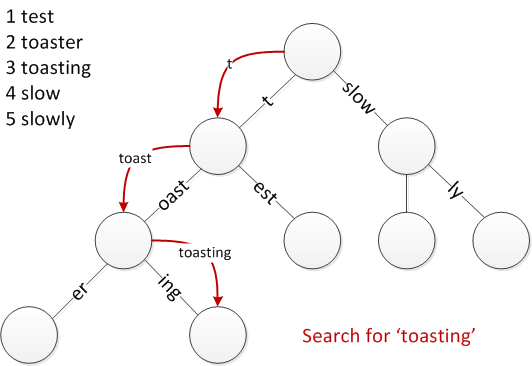
\includegraphics[width=1\textwidth]{immagini/patricia_trie.png}
\caption{Struttura di patricia trie}
\label{fig:mesh6}
\end{figure}

Patricia Tree facilità l'inserzione, l'eliminazione e l'aggiornamento di dati, obiettivi importanti per questioni di efficienza in una situazione dove lo stato della rete necessita di aggiornamenti frequenti. Per una descrizione formale dei vantaggi inerenti a questa struttura dati si rimanda all’appendice D, “Modified Merkle Patricia Tree” del Yellowpaper Ethereum\footfullcite{ethYellowpaper}.

\subsection{Ethereum Metropolis e Constantinople}

Sezione (forse) opzionale, scrivo della transizione in corso da PoW a PoS in Ethereum, l'aggiunta di EiP (Ethereum imporvement Proposals) per contrastare problemi di scalabilità con vari miglioramenti, per esempio EVM diventa più efficiente ecc. 
È un fork quindi posso brevemente spiegare la differenza tra soft e hard forks.

\section{Smart Contracts}

Una delle potenzialità più promettenti di Ethereum deriva dall’implementazione di un linguaggio di programmazione Turing completo, il quale permette di scrivere contratti (intelligenti) chiamati per l’appunto Smart Contracts. Il termine è stato coniato da Nick Szabo, nel 1994 che lo definisce come "protocollo di transazione computerizzato che esegue i termini di un contratto"\footfullcite{SzaboSmartContract}. Una definizione sempre attuale che nel caso del paradigma, soggetto di questa tesi, può essere espressa come contratto o programma immutabile situato direttamente sulla blockchain. Come già detto nella sezione precedente i contratti fanno parte dello stato della rete e quindi hanno un vero e proprio indirizzo con la possibilità di effettuare operazioni automatiche. Quando sono soddisfatte le
certe condizioni descritte nel codice, vengono automaticamente avviate specifiche azioni, anch'esse definite nel codice.

\subsection{Solidity}

\subsection{Ethereum Virtual Machine}

\subsection{Gas}

\section{Data storage}